\RequirePackage{tikz}

\documentclass{article}
\usepackage[utf8]{inputenc}

\title{Playground}
\author{alena.beyer }
\date{February 2017}

\usetikzlibrary{shadows,shadings,shapes.symbols}
\tikzset{
    double color fill/.code 2 args={
        \pgfdeclareverticalshading[%
            tikz@axis@top,tikz@axis@middle,tikz@axis@bottom%
        ]{diagonalfill}{100bp}{%
            color(0bp)=(tikz@axis@bottom);
            color(50bp)=(tikz@axis@bottom);
            color(50bp)=(tikz@axis@middle);
            color(50bp)=(tikz@axis@top);
            color(100bp)=(tikz@axis@top)
        }
        \tikzset{shade, left color=#1, right color=#2, shading=diagonalfill}
    }
}

\begin{document}

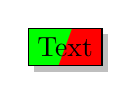
\begin{tikzpicture}[my node/.style={draw, rectangle, cloud ignores aspect, drop shadow, double color fill={green}{red}}]

\node[my node, shading angle=70]  at (0,0) {Text};
%\foreach \angle[count=\i] in {0,15,...,75} \node[my node, shading angle=\angle] (a\i) at (0,\i) {Text};
%\foreach \angle[count=\i] in {105,120,...,180} \node[my node, shading angle=\angle] (b\i) at (3,\i) {Text};
%\path (a6) -- node[my node, shading angle=90]{Text} (b1);
\end{tikzpicture}

\end{document}
